\documentclass[../main.tex]{subfiles}
\setlength{\parindent}{10pt}

\begin{document} \noindent
The aim of the current study was to characterize entrainment and resonance properties in the visual cortex in absence and presence of gamma-band oscillations induced by visual gratings. 
To this end, we drove the visual cortex with a rapid flicker at frequencies ranging from 52 to 90 Hz, in steps of 2 Hz. The photic drive was applied either to a circular patch (the \RFTonly condition, Figure \ref{fig:paradigm}A,C) or to the light gray rings of a moving grating stimulus (the \gammaRFT condition, Figure \ref{fig:paradigm}B,D). We hypothesized that a photic drive in the \gammaRFT condition would entrain the grating-induced oscillations. This would be observed as the endogenous gamma oscillation synchronizing with the flicker. \textcolor{red}{Synchronization would be reflected by a constant phase angle between the neuromagnetic signal and the stimulation ('phase entrainment'), as well as a reduction in power at the IGF, indicating a change in the peak frequency of the gamma oscillator towards the flicker frequency \citep['frequency entrainment';][]{pikovsky2003synchronization}.} Moreover, we expected the presence of the induced gamma oscillator to change the resonance properties (compared to the \RFTonly condition), reflected by an amplification of responses to stimulation frequencies equal to the endogenous gamma rhythm. Response magnitudes in the \RFTonly condition were expected to reveal resonance properties of the visual system in absence of gamma oscillations, demonstrating favorable stimulation frequencies to be used in future experiments applying Rapid Frequency Tagging \citep[RFT;][]{zhigalov2019probing,drijvers2020rapid}.

\subsection{Identifying Individual Gamma Frequencies} \label{IGF} \noindent
The frequency of the endogenous gamma rhythm is known to vary between participants \citep{hoogenboom2006localizing,hoogenboom2010visually,muthukumaraswamy2010visual,van2012magnetoencephalography}. 
Therefore, each subject's Individual Gamma Frequency (IGF) was identified first, based on the 0 - 2 s interval in the \gammaRFT condition during which the moving grating stimuli were presented without the visual flicker (Figure \ref{fig:paradigm}C). The Time-Frequency Representations (TFRs) of power are depicted in Figure \ref{fig:IGF_example}A,B for two representative participants. The center column shows the power averaged over time (0.25 - 1.75 s after the stimulus onset to avoid any event-related field confounds) demonstrating distinct peaks at 58 and 74 Hz for these participants. The topographies in the right column depict relative power change at the identified frequencies, focally in sensors over the occipital cortex. For each subject, the 2 - 3 combined planar gradiometers showing maximum relative power change in the gamma band were selected for further analysis (Sensors-of-Interest; SOI) per visual inspection. These sensors strongly overlapped between participants. The data of participants with an IGF closer than 6 Hz to the lowest (52 Hz) drive, i.e. IGF$<$58 Hz, were not considered for further analyses. 
\begin{figure}[H]
    \centering
    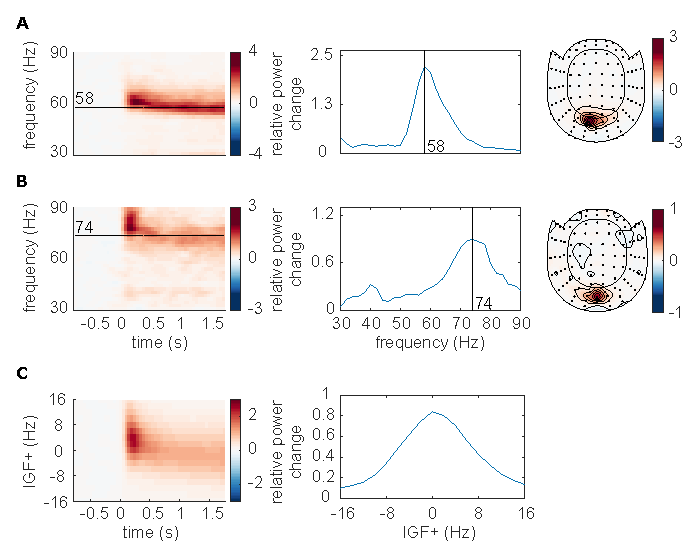
\includegraphics[width=115mm]{figures/fig2_IGF.eps}
      \captionsetup{width=115mm}
    \caption[Identification of Individual Gamma Frequencies (IGF) and Sensors-of-Interest (SOI)]{Identification of Individual Gamma Frequencies (IGF) and Sensors-of-Interest (SOI). \textbf{A, B} The TFRs of power, power spectra (averaged over 0.25 - 1.75 s) and topographic representations (combined planar gradiometers) of the IGF for two representative participants. The TFRs of power were calculated from the Fourier Transforms using a 500 ms sliding window, resulting in spectral smoothing of $\pm$3 Hz. The IGFs were identified from the spectral peak in 0.25 - 1.75s interval of the TFRs. Identified IGFs are indicated by dashed lines. \textbf{C} The grand-average of the power analysis after aligning the individual TFRs and spectra to the IGF (N=22).}
    \label{fig:IGF_example}
\end{figure}

Figure \ref{fig:IGF_example}C depicts the averaged TFRs of power as well as the power spectrum for the remaining subjects (N=22), aligned to each participant's IGF prior to averaging. The moving grating stimulus induced sustained oscillatory activity constrained to the IGF $\pm$ 8 Hz, with an average relative power change of 80\% in the 0.25 - 1.75 s interval compared to baseline. In short, the moving gratings produced robust gamma oscillations observable in the individual participants which reliably allowed us to identify the individual gamma frequencies. 

\subsection{Photic drive induces responses up to $\sim$80 Hz} \noindent
We next set out to quantify the rhythmic response to the flicker as a function of frequency in the \RFTonly condition, in which stimulation was applied to an invisible patch. Figure \ref{fig:RFT_example} A and B, left panel, depicts the overlaid power spectra for the different stimulation frequencies in two representative participants (the same as in Figure \ref{fig:IGF_example}). The spectra were estimated by averaging the TFRs of power in the 0.25 - 1.75s interval after flicker onset. Due to the overlap of the sensors detecting the gamma oscillations and photic drive response (compare Figure \ref{fig:IGF_example} and \ref{fig:RFT_example} right columns) the same SOI were used as in the \gammaRFT condition.
Both individuals showed strong responses at the respective stimulation frequencies, with a maximum relative power change of 200\% and 500\% in subject A and B, respectively. \textcolor{red}{The identified IGFs (indicated by vertical dashed lines) were higher than the frequencies inducing the strongest flicker response in 20 out of 22 participants (exact Binomial Test against H_{0}, hyopthesizing a p-value of 0.5: $p = 0.00012, probability of successes (IGF>flicker freq) 0.91, Bayes Factor BF_{10}=309.3$).} When averaged over all participants, the magnitude of the flicker response decreased systematically with frequency (Figure \ref{fig:RFT_example}\textbf{C}).
\begin{figure}[H]
   \centering
    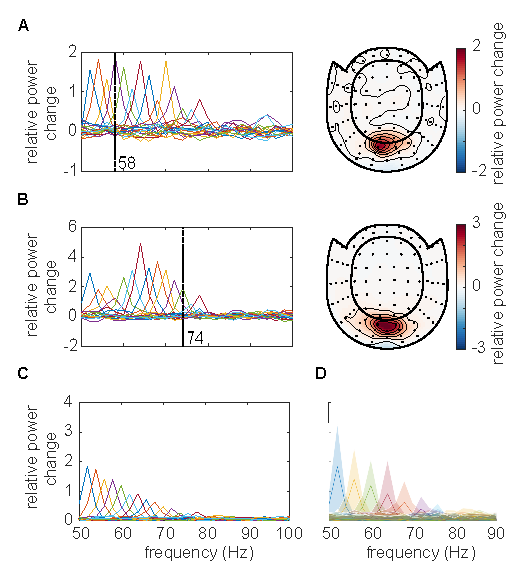
\includegraphics[width=85mm]{figures/fig3_flicker.eps}
      \captionsetup{width=85mm}
    \caption[Topographies of the response to the rhythmic flicker]{\textbf{A,B} The response to the photic drive in the \RFTonly condition and the corresponding topographies for two representative subjects. Spectra were estimated from the TFRs of power averaged in the 0.25 - 1.75 s interval. Dashed vertical lines indicate the participants' IGF. The topographies (combined planar gradiometers) demonstrate a strong overlap with the ones in Figure \ref{fig:IGF_example}. \textbf{C} Grand-average of the responses to the photic drive for each flicker frequency. On average, the magnitude of the flicker response decreases with increasing frequency, and is identifiable for stimulation below 80 Hz. \textbf{D} Grand-average flicker responses for frequencies from 52 to 90 Hz in steps of 4 Hz. The shaded areas, illustrating the standard deviation, indicate a substantial inter-subject variability.}
    \label{fig:RFT_example}
\end{figure}

Figure \ref{fig:av_res}A displays the power spectra in the \RFTonly condition, estimated from the TFRs as explained above, averaged over all participants, as a function of stimulation frequency. These are equivalent to \ref{fig:RFT_example}C. Diagonal values indicate the magnitude of the oscillatory responses (relative to baseline) at the stimulation frequencies, reaching values of up to 300\% and decreasing monotonically with frequency. This confirms an upper limit for the stimulation of around 80 Hz. Off-diagonal values indicate oscillatory activity at frequencies different from the stimulation frequency. Figure \ref{fig:av_res}B shows the same spectra after aligning to the individual IGFs, prior to averaging.
Figure \ref{fig:av_res}C and D display the spectra in the \gammaRFT condition (averaged in the 2.25 - 3.75s interval), during which the photic drive was applied to the moving grating stimulus (see Figure \ref{fig:paradigm}B). The induced gamma band activity can be observed as the horizontal light red band at $\sim$60 Hz. When aligning the spectra to the IGF (Figure \ref{fig:av_res}D),  we observe a decrease in the flicker response but no evidence for an amplification at or close to the IGF.

\begin{figure}[H]
    \centering
    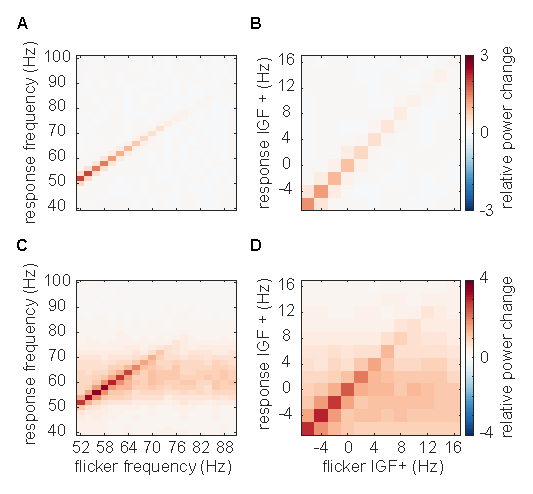
\includegraphics[width=85mm]{figures/fig4_av_power.eps}
    \captionsetup{width=85mm}
    \caption[Averaged power spectra per \textit{frequency}$\times$\textit{condition} combination]{Average relative power change to the photic drive (y-axis) with respect to the driving frequencies (x-axis) \textbf{A} The \RFTonly condition. Note that the power changes mirror Figure \ref{fig:RFT_example}\textbf{C}. Power decreases with increasing frequency, from a relative change of $\sim$3 at 52 HZ to $\sim$.5 at 80 Hz. \textbf{B} The \RFTonly condition after the spectra were aligned to the IGF. \textbf{C} The \gammaRFT condition. All spectra demonstrate both the flicker response and induced gamma oscillation (observed as the light red horizontal band). Again, the amplitude of the rhythmic stimulation response appears to decrease with increasing frequency. \textbf{D} The spectra for the \gammaRFT condition now aligned to the IGF. There is no indication that the rhythmic flicker captures the endogenous gamma oscillations.}
    \label{fig:av_res}
\end{figure}

\subsection{Magnitude of flicker response decreases as a function of frequency} \noindent
The averaged TFRs of power in Figure \ref{fig:av_res} point to an approximately linear decrease in power of the flicker response with increasing frequency. Literature on neural resonance and entrainment, however, suggests the existence of a preferred rhythm at which oscillatory responses are amplified \citep{hutcheon2000resonance,herrmann2001human,pikovsky2003synchronization,notbohm2016modification,gulbinaite2019attention}. As argued in \citet{pikovsky2003synchronization} phase-locking between the driving signal and the self-sustained oscillator is the most appropriate metric to investigate entrainment. Figure \ref{fig:freq_fun}A,B depicts the phase-locking value (PLV) between the photodiode and the MEG signal at the SOI (planar gradiometers, not combined). This measure reveals a systematic decrease in phase-locking with increasing flicker frequency for both the \RFTonly (orange) and \gammaRFT (blue) condition (A). The observed relationship is preserved when aligning the frequencies to the IGF (B, also see Table \ref{table: linregr}). Note the absence of increased phase-locking at the IGF. The magnitude of the flicker response, quantified by power change compared to baseline, as a function of frequency, is demonstrated in Figure \ref{fig:freq_fun}C-F and depicts a similar relationship to the one observed for the PLV. The \RFTonly condition (C, orange line) revealed a systematic decrease with frequency, whereas the \gammaRFT condition did show a peak at 56 Hz. However, this observed increase appeared to be caused by considerable variance between the power estimates of the individual participants (see Figure \ref{fig:freq_fun}E, each line graph depicts power estimates per individual participant). We again aligned the spectra to the IGF before computing the grand-average (Figure \ref{fig:freq_fun}D). The absence of a peak at 0 Hz suggests no evidence for resonance at the IGF, confirming the peak at 56 Hz in C to be the result of inter-subject variability. Indeed, simple linear regression models, fit individually to PLV and power as a function of frequency aligned to the IGF, separately for each condition, explain a considerable amount of the variance (see Table \ref{table: linregr} and dotted lines in Figure \ref{fig:freq_fun}). We then identified the individual peak frequencies, eliciting the strongest response to the flicker in the \gammaRFT condition \ref{fig:freq_fun}E, and related those to the IGF, as seen in Figure \ref{fig:freq_fun}F. \textcolor{red}{As observed in the flicker condition, the frequency inducing the strongest response to the flicker was lower than the IGF in the majority of participants, i.e. 19 out of 22 (exact Binomial Test against $H_0: p = 0.0008$, Bayes Factor $BF_{10} = 67.5$).}

\begin{figure}[H]
\centering
    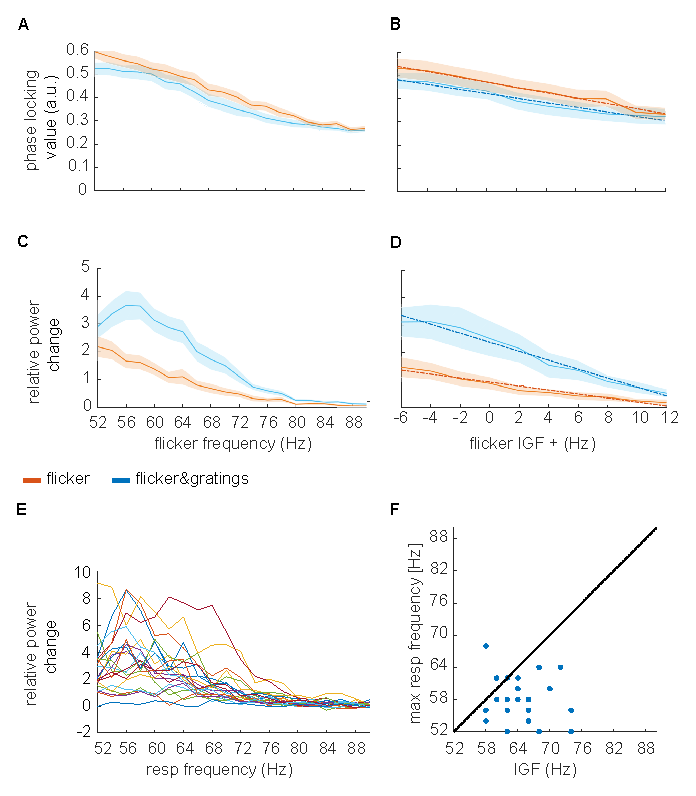
\includegraphics[width=115mm]{figures/fig5_freq_fun.eps}  
    \captionsetup{width=115mm}
    \caption[Magnitude of the flicker response as a function of frequency]
    {Magnitude of the flicker response as a function of frequency in the \RFTonly (orange) and \gammaRFT (blue) condition. Shaded areas indicate the standard deviation. \textbf{A} The phase-locking values between the photo-diode and the MEG signal over the SOIs as a function of driving frequency. \textbf{B} The phase-locking values between the photo-diode and the MEG signals as a function of frequency after the spectra were aligned to the IGF. Again, the phase-locking decreases with increasing frequency (see Table \ref{table: linregr} for a statistical quantification of the simple linear regression models). \textbf{C} Relative power change with respect to baseline as a function of frequency. Generally, the power decreased with frequency, however, in the \gammaRFT there is an apparent peak at $\sim$56 Hz. The shaded area (standard deviation) indicates considerable variance between participants. \textbf{D} Relative power change as a function of frequency after the individual spectra were aligned in frequency according to the IGF, demonstrating that responses to a photic drive at the IGF are not amplified. \textbf{E} Relative power change as a function of frequency for each individual subject (N = 22), indicates that the peak at $\sim$56 Hz in \textbf{C} is driven by comparably high power in that frequency range in just a few individuals. \textbf{F} Flicker frequency inducing highest power values versus IGF, demonstrating the IGF to be higher than the  frequency inducing maximum power change in the majority of participants.}
    \label{fig:freq_fun}
\end{figure}

\begin{table}[H]
\begin{minipage}[b]{90mm}\centering
\captionsetup{width=90mm}
\caption[Estimated simple linear regression models: Flicker response as a function of frequency]{Simple linear regression models: Flicker response magnitude as a function of distance to IGF.}
\label{table: linregr}
   \begin{tabular}{r r r r r r r}
    \toprule
        \multicolumn{1}{l}{\textbf{Model}} & \multicolumn{5}{l}{{\textbf{Estimates}}} \\ 
        {} & {$\beta\textsubscript{1}$} & {t} & {p \text{***}} & {$R^2$} & {F(1,218)}\\ 
        \hline
        \RFTonly_{plv} & $-.01$ & $-8.07$ & $<2.2e-16$ & $.23$ & $65.07$ \\
         \gammaRFT_{plv} & $-.01$ & $-7.24$ & $<2.2e-16$ & $.19$ & $52.44$  \\
        \RFTonly_{pow} &$-.07$ & $-9.01$ & $4.80e-14$ & $.27$ & $81.14$ \\
        \gammaRFT_{pow} &$-.16$ & $-8.95$ & $7.51e-12$ & $.27$  & $80.13$  \\

        \bottomrule
    \end{tabular}   
% df = 22 subj*10freq
\end{minipage}
\end{table}


\subsection{Gamma oscillations and flicker response coexist} \noindent
We initially hypothesized that entrainment of the gamma oscillations in the \gammaRFT condition would result in the photic drive capturing the oscillatory dynamics when the driving frequency was close to endogenous gamma oscillations. Figure \ref{fig:subj_ent} depicts the TFRs of power relative to a 0.5 s baseline, for one representative subject (also shown in Figure \ref{fig:IGF_example} and \ref{fig:RFT_example}A). The averaged trials for a photic drive at 52 Hz are shown in Figure \ref{fig:subj_ent}A and separately for each flicker frequency in Figure \ref{fig:subj_ent}B \citep[Figure created using function by][]{tightsub}. The IGF (58 Hz for this subject) and the respective stimulation frequencies are indicated by dashed lines. The endogenous gamma oscillations, induced by the moving grating stimulus, are observed as the sustained power increase from 0 - 6 s whereas the flicker response is demonstrated by a power increase at 2 - 4 s. The plots reveal that gamma oscillations persist at the IGF and coexist with the response to the photic drive, which is particularly apparent for stimulation at 52 Hz (Figure \ref{fig:subj_ent} A). Furthermore, the power increase at the flicker frequency does not appear to outlast termination of the drive at t = 4 s. In the subsequent step, we frequency-aligned the TFRs of power according to the IGF before averaging over participants. Again, the analyses were constrained to individuals with an IGF above 56 Hz (N = 22).
\begin{figure}[H]
    \makebox[\textwidth][c]{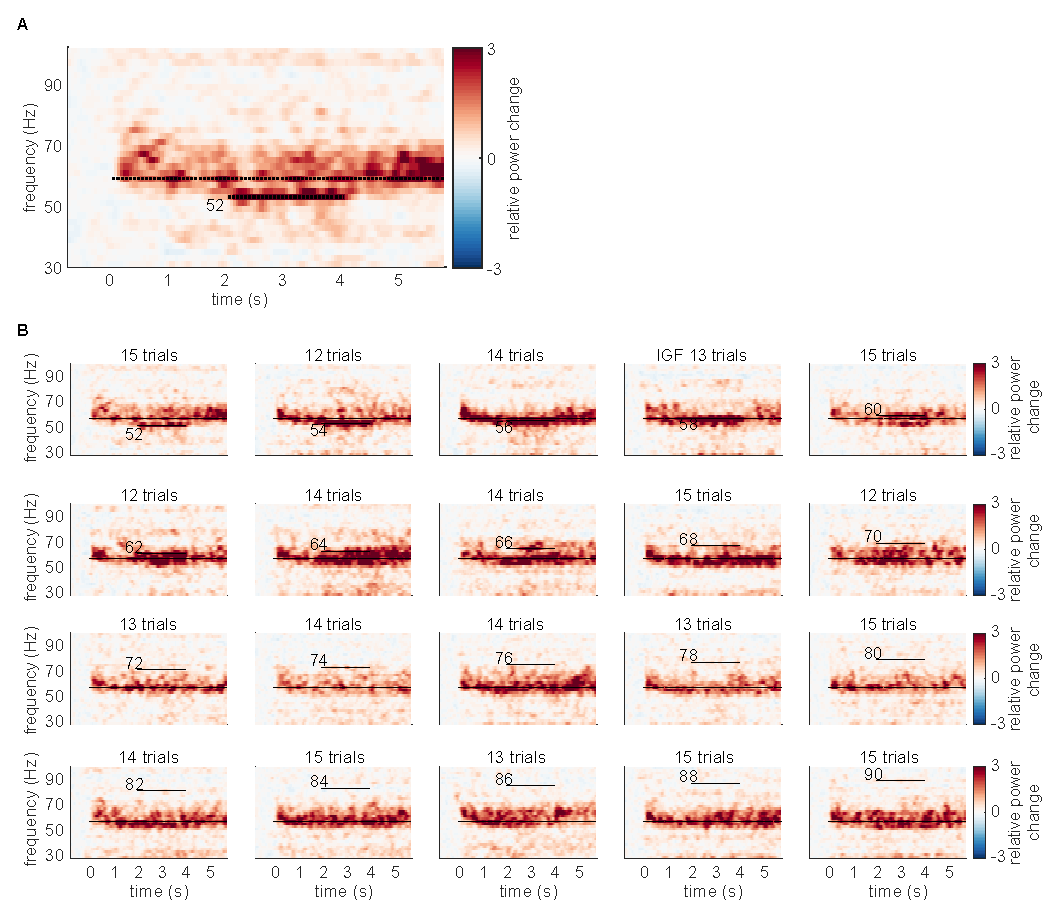
\includegraphics[width=176mm]{figures/fig6_singsubj_TFR.eps}}
    \captionsetup{width=176mm}

    \caption[Single-subject Time-Frequency Representations of the \gammaRFT condition]{The time-frequency representations (TFRs) of power for one representative subject, showing relative power change averaged over trials and SOIs in the \gammaRFT condition.  \textbf{A} Photic drive at 52 Hz. The moving grating stimuli were presented for 0 - 6 s, with the flicker superimposed from 2 to 4 s. Sustained gamma-band activity is clearly observable throughout the presentation of the stimuli, with a power increase of 300\% relative to baseline. Additionally, the rhythmic stimulation elicited a response at 52 Hz, which seems to coexist with the gamma oscillations, indicating that the photic drive is unable to capture the dynamics of the gamma oscillation.  \textbf{B} The plots for the frequencies from 52 to 90 Hz. Stimulation frequencies and IGF (here 58 Hz) are indicated by horizontal dashed lines. The flicker induced responses up to 66 Hz in this participant. Gamma oscillations persist in presence of flicker responses, suggesting that they coexist.}
    \label{fig:subj_ent}
\end{figure}
The group averaged, aligned TFRs are shown in Figure \ref{fig:TFRGA_ent} for frequencies ranging from IGF-6 Hz to IGF+16 Hz. The endogenous gamma oscillations are observed as the power increase extending from 0 - 6 s, and the flicker response as the power change in the 2 - 4 s interval marked by dashed lines, respectively. The photic stimulation induces a reliable response that decreases toward 12 Hz above the IGF. Despite the representation of the gamma oscillations being smoothed due to inter-individual differences, the averaged aligned TFRs of power support the observations in the single subject data: both the gamma oscillations and flicker response coexist in the 2 - 4 s interval. Furthermore, there is no indication of the gamma power being reduced during RFT at frequencies close to, but different from, the IGF.
\begin{figure}[H]
\centering
    \makebox[\textwidth][c]{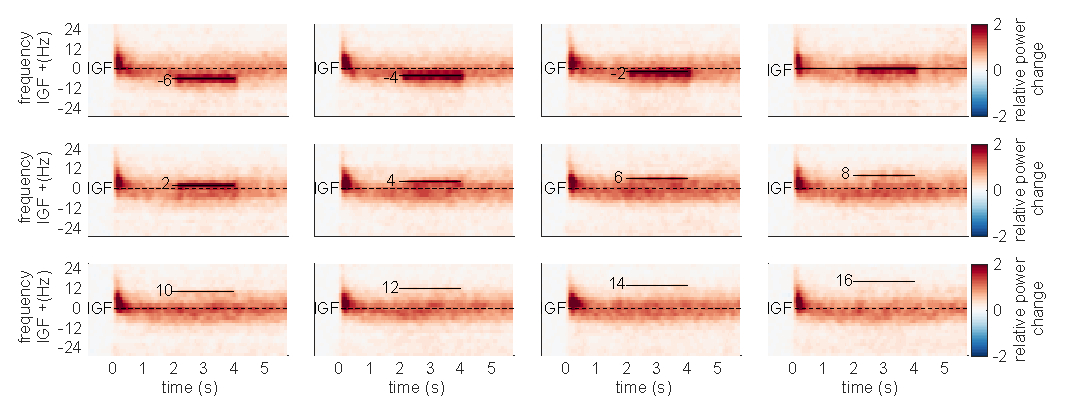
\includegraphics[width=176mm]{figures/fig7_GA_TFR.eps}} 
    \captionsetup{width=176mm}
    \caption[Grandaverage Time-Frequency Representations of the \gammaRFT condition]{Grand-average TFRs of power after aligning to the IGF for each subject in the \gammaRFT condition. The stimulation frequencies (from -6 to 16 Hz relative to the IGF) are indicated by dashed horizontal lines. As suggested by the single subject TFRs in Figure \ref{fig:subj_ent}, the endogenous gamma oscillations and the flicker response seem to be coexistent. Thus, there is no obvious indication of the photic drive being able to capture the dynamics of the gamma oscillations.}
    \label{fig:TFRGA_ent}
\end{figure}

\textcolor{red}{In addition to the narrow-band gamma oscillations, the gratings elicited a rhythmic response at 4 Hz, i.e. the velocity of the concentric drift (not shown). Apart from that, we did not find any evidence for an intermodulation between the frequency of the movement and the photic drive.}

\subsection{\textcolor{red}{Frequency analyses with a longer time window confirm robustness of the reported results}} \textcolor{red}{To assess the robustness of our results, we repeated the frequency analyses in the \RFTonly and \gammaRFT condition with a 2s sliding time window. The longer window substantially increased the signal-to-noise ratio of the flicker response, to up to over 400\% relative power change in the \RFTonly condition and more than 600\% in the \gammaRFT condition (not shown). Besides that, the analyses replicated our reported main finding: a reduction in response magnitude (power) with increasing frequency, in both conditions, following the same trend as depicted in Figure \ref{fig:freq_fun}C and D. The 2 s sliding time-window did however not optimally capture the gamma power, which has a broader peak than the response to the photic drive. The 500 ms sliding window used in our reported analyses is therefore a good compromise, allowing both a reliable identification of a gamma peak frequency and a sufficiently high signal-to-noise ratio and frequency resolution of the flicker response (see Figure \ref{fig:subj_ent}A).}

\subsection{\textcolor{red}{Oscillatory gamma dynamics cannot be captured by frequency entrainment}} \noindent \textcolor{red}{Synchronisation of neuronal oscillations by rhythmic stimulation could be conceptualized as the entrainment of a self-sustained oscillator by an external force \citep[e.g.][]{notbohm2016modification,helfrich2019neural}; resulting in a change in frequency of the ongoing oscillations, so-called 'frequency entrainment'. Visual inspection of the TFRs of power in Figure \ref{fig:subj_ent} and \ref{fig:TFRGA_ent} do no indicate any modulation of the peak frequency of the gamma oscillations by the flicker response, suggesting that they do not synchronize. To quantify these observations, we investigated the power of the gamma oscillations before and during the photic drive (Figure \ref{fig:boxpl_ent}) in the \gammaRFT condition.} A central assumption of oscillatory entrainment is the existence of a 'synchronization region' in the frequency range around the endogenous frequency of the oscillator, the so-called Arnold tongue \citep[e.g.][]{pikovsky2003synchronization}. Driving frequencies falling inside this synchronization region, will be able to modulate the dynamics of the self-sustained oscillator \citep[also see][]{hutt2018effect}. \textcolor{red}{With this in mind, the following analyses only included flicker frequencies in the vicinity of the IGF.} For each participant, we considered the relative power change induced by the moving gratings in the 0.5 - 1.5 s interval (T1) before the flicker onset and in the 2.5 - 3.5 s interval (T2) in which both the moving gratings and the photic drive were present. We investigated this for stimulation frequencies below the IGF (averaged power for -6 and -4 Hz) and above (averaged power for +4 and +6 Hz). Assuming a symmetric Arnold tongue centered at the IGF, as shown for entrainment in the alpha-band \citep{notbohm2016modification}, we expected a reduction in power at the IGF in interval T2 compared to interval T1 for both higher and lower driving frequencies, i.e. an effect of time, but not frequency. Figure \ref{fig:boxpl_ent} depicts power change at the IGF for the factors stimulation frequency (drive$<$IGF and drive$>$IGF) and time interval (T1 and T2), averaged over the SOIs for each subject. In accordance with the TFRs in Figure \ref{fig:TFRGA_ent}, there is no meaningful indication for gamma power being reduced during the T2 interval as compared to the T1 interval, affirming the coexistence of the two responses. \textcolor{red}{A factorial repeated-measures ANOVA did not reveal any significant main effects of the factors time (T1 vs T2) and frequency (drive$<$IGF vs drive$>$IGF), but a significant interaction effect ($F(1,21)=5.09, p=0.003, \eta^2=.003$). These results were further investigated using a Bayesian repeated-measure ANOVA. The obtained Bayes factors ($BF_{10}$) indicate that the variance in the data underlies the variability between participants, while the factor \textit{time} ($BF_{10} = 0.233$) and both \textit{time} and \textit{frequency} ($BF_{10} = 0.274$) do not add any explanatory value. Evidence for the interaction effect \textit{time:frequency} was found to be inconclusive ($BF_{10} = 0.53$), as was the main effect of frequency alone $BF_{10} = 1.146$). These results provide evidence against the expected reduction in gamma power during rhythmic photic stimulation at frequencies different from the IGF; suggesting that the flicker did not capture the oscillatory gamma dynamics.}

\begin{figure}[H]
    \centering
    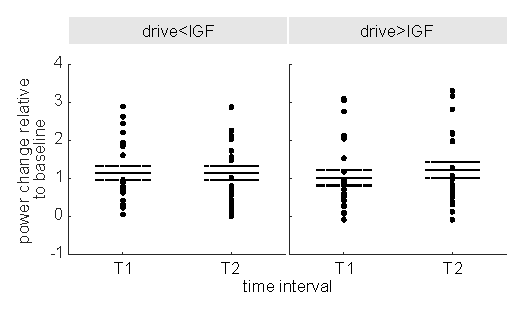
\includegraphics[width=85mm]{figures/fig8_powchan_abobel.eps}  
    \captionsetup{width=85mm}
    \caption[Power change at the IGF as an indicator of frequency entrainment]{Power change relative to baseline at IGF in response to the moving grating stimuli before (T1; 0.5 - 1.5 s) and during application of the flicker (T2; 2.5 - 3.5 s), at frequencies below and above IGF (drive$<$IGF [-6, -4 Hz] and drive$>$IGF [+4, +6 Hz], respectively). Scatters demonstrate individual values, solid and dashed lines depict mean and standard deviation, respectively. The key finding is that power at T2 is not decreased compared to T1 for either of the frequency ranges, which is supported by a Bayesian repeated measures ANOVA ($BF_{10} = 0.274$).}
    \label{fig:boxpl_ent}
\end{figure}

\subsection{Photic drive does not reliably modulate gamma phase} \noindent
Synchronization of a self-sustained oscillator by an external force, i.e. entrainment, is reflected by a constant phase angle between the two oscillators over extended intervals, so-called \textit{phase plateaus}. These might occur when the frequency of the driver is close to the endogenous frequency of the oscillator, i.e. within its Arnold Tongue \citep{rosenblum2000detection,pikovsky2003synchronization,notbohm2016modification}. When approaching the edge of the synchronization region, episodes of constant phase angles are interrupted by so-called \textit{phase slips} that emerge when the self-sustained oscillator briefly unlocks from the driving force and oscillates at its own frequency. These phase slips will be observed as steps between the phase plateaus. \textcolor{red}{The phase plateau analysis was implemented to complement the PLV analysis shown in Figure \ref{fig:freq_fun}. The PLV quantifies the average synchrony between photodiode and neuromagnetic signal over trials using a 500 ms sliding time window. We hypothesized that in the case of oscillatory entrainment, the gamma oscillator in the \gammaRFT condition would alternate between locking on to the photic drive for a few cycles and slipping back to its endogenous rhythm. Due to the short duration of the gamma cycle ($\sim$17.2 ms for a 58 Hz IGF), this intermittency would be smeared out by the sliding window. As there was no endogenous gamma oscillator in the flicker condition, such an intermittency was not expected.} To investigate phase entrainment of the gamma oscillations by the photic drive, we inspected the phase angle between the photodiode and one, individually selected, occipital gradiometer of interest per participant. The time series of the phase were estimated per trial, separately for the two sensors, using a sliding time-window Fourier transform approach ($\Delta$T = 3 cycles = 3/$f_{flicker}$s; Hanning taper). Phase differences per trial were obtained by subtracting the unwrapped phase angle time series.

\paragraph{Phase angle between photodiode and MEG signal over time} 
Figure \ref{fig:plat_singlesubj} illustrates the unwrapped phase angles between the MEG and photodiode signal during the photic drive at the IGF (here 58 Hz), in the \RFTonly (A) and \gammaRFT condition (B), respectively, for the same representative participant shown in Figure \ref{fig:IGF_example}A, \ref{fig:RFT_example}A and \ref{fig:subj_ent}. The colored line graphs depict individual trials. In both conditions, the MEG signal drifts apart from the photic drive, towards a maximum difference of 60 radians, i.e. a phase difference of about 9.5 cycles, by the end of the trial (A and B, top panel). Interestingly, the direction of the phase angle appears to change during some of the trials, suggesting spectral instability of the gamma oscillations. Furthermore, the graphs demonstrate a substantial inter-trial variability. This diffusion between trials, quantified for each participant as the standard deviation over trials at the end of the photic stimulation (t=2 in \RFTonly and t=4 in \gammaRFT condition), converted from radiant to ms, is juxtapositioned in Figure \ref{fig:plat_singlesubj}C for the two conditions. It can be readily seen that the phase angles between the stimulation and MEG signal fan out highly similarly in absence and presence of the endogenous gamma oscillations.
\paragraph{Phase plateaus}
Visual inspection of the first 0.25 s of the phase angle times series, depicted in Figure \ref{fig:plat_singlesubj}A,B lower panel, does not suggest a relatively high number of phase plateaus in the \gammaRFT compared to the \RFTonly condition, that would have been expected if the photic drive was able to entrain the endogenous gamma oscillator. Importantly, the graphs demonstrate the phase angles to reach values of over 2$\pi$, i.e. more than one cycle, within the duration of the first gamma cycle (17.2 ms), suggesting that even stimulation at the endogenous frequency of the oscillator cannot capture the gamma dynamics. To verify these observations for the entire sample, plateaus during stimulation at the IGF were identified based on the mean absolute gradient ($\leqslant$0.01 rad/ms, see equation \ref{eq:plat}) over the duration of one cycle of stimulation, i.e. 18 consecutive samples for a flicker frequency of 58 Hz. Figure \ref{fig:plat_singlesubj}D shows the average number of plateaus per trial as a function of flicker frequency aligned to IGF, averaged over participants. The shaded areas indicate the standard deviation. While the \gammaRFT condition exhibits more phase plateaus than \RFTonly for all stimulation frequencies, the number of plateaus decreases similarly in both conditions with increasing frequency. Importantly, stimulation at the IGF did not result in the highest number of plateaus in either condition. \textcolor{red}{These results are in line with the reported frequency analyses: responses to the photic drive in \gammaRFT show strong similarity to the \RFTonly condition despite the presence of the gamma oscillator.} The results affirm the observations presented in Figure \ref{fig:freq_fun}A and B. 

\begin{figure}[H]
\centering
    \makebox[\textwidth][c]{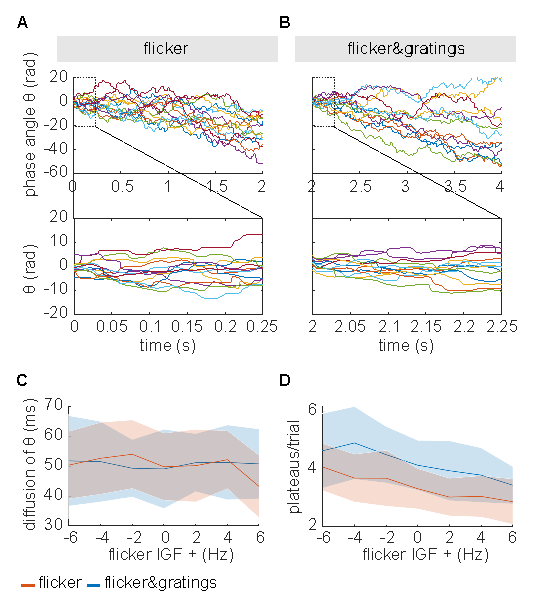
\includegraphics[width=85mm]{figures/fig9_plateau.eps}} 
    \captionsetup{width=85mm}
    \caption[Phase angle and phase plateaus]{\textbf{A,B} Phase angle between photodiode and the MEG signal (one gradiometer of interest) at the IGF, for one representative participant; colored lines depict individual trials.
    \textbf{A} Phase angle $\theta$ in the \RFTonly condition over duration of the flicker presentation (upper panel) and the first 250 ms (lower panel). The MEG signal drifts apart from the stimulation and can reach a maximum accumulated phase difference of 60 rad, i.e. 9.54 cycles, at the end of the stimulation and up to 15 rad, i.e. 2.39 cycles, in 250 ms.
    \textbf{B} The increase in phase difference over the time of the stimulation for the \gammaRFT condition (upper panel) and in the first 250 ms (lower panel). The diffusion of the phase difference across trials is similar to the \RFTonly condition. Moreover, there is no clear difference in the number and length of phase plateaus between conditions, implying that the presence of the gamma oscillations does not facilitate entrainment at the IGF. \textbf{C} Fanning out across trials as a function of frequency aligned to IGF. Trials diffuse to a highly similar extent in both conditions and across frequencies. \textbf{D} Number of plateaus per trial as a function of frequency. While the \gammaRFT conditions exhibits more plateaus for all flicker frequencies, there is no indication that stimulation at the IGF results in comparably strong synchronization.}
    \label{fig:plat_singlesubj}
\end{figure}

\textcolor{red}{
\subsection{The sources of the gamma oscillations and the flicker responses peak at different locations} \noindent
The coexistence of the endogenous gamma oscillations and flicker response suggest that these two signals are generated by different neuronal populations; possibly in different regions. To test this assumption we localized the respective sources using Linearly Constrained Minimum Variance spatial filters \citep[LCMV;][]{van1997localization}. The covariance matrix for the spatial filters was estimated based on the -0.75 to -0.25 s baseline in both conditions, the 0.75 to 1.25 s interval with the moving gratings in \gammaRFT and the invisible flicker in the \RFTonly condition, as well as the 2.75 to 3.25 interval in the \gammaRFT condition in which the flicker was applied to the grating stimulus. Note that for each participant, one common filter was used for source estimation in both conditions. Power values at the IGF and flicker frequencies, averaged up to 78 Hz, respectively for the \gammaRFT and \RFTonly condition, were estimated based on the Fourier Transform. To extract power at the IGF and flicker frequencies, power change was computed relative to the baseline interval at each of the 37,163 grid points using equation \ref{eq:rlc}. To isolate the flicker response on the \gammaRFT condition, the flicker\&gratings interval was contrasted to the moving grating interval. 
Figure \ref{fig:sourceGA} illustrates the grandaverage of the source localization for the gamma oscillations (A), the invisible flicker response (B) and the response to the flickering gratings (C). Consistent with previous work, the responses originate from mid-occipital regions \citep{hoogenboom2006localizing,zhigalov2019probing}. It is worth noting that the sources of the gamma oscillations and response to the invisible flicker are relatively focal, while the activity induced by the flickering gratings extends more broadly over visual cortex. Using the MNI to Talaraich mapping online tool by Biomag Suite Web (MNI2TAL Tool) \citep[see][]{lacadie2008brodmann,lacadie2008more}, the peak of the gamma oscillations was located in the ventral part of the secondary visual cortex (V2, Brodmann area 18; MNI coordinates = [-6mm -100mm -8mm], grandaverage). The peak sources of the flicker responses in both conditions were found in the Calcarine Fissure, at a 2mm distance to the border of the primary (V1) and secondary visual cortex (in dorsal direction), suggesting that they are generated by neighboring, coherent sources in both hemispheres in and close to V1 \citep{belardinelli2012source} (MNI coordinates: flicker [6mm -96mm 12mm]; flicker\&gratings [6mm -100mm 0mm]). 
To compare the peak locations between the sources in a lower dimensional space, the identified 3D coordinates were projected along their first Principal Component \citep{herrmann2011syntactic}. Dependent sample t-tests revealed a significant difference in location between the peak sources of the IGF and the invisible flicker responses $t(21) = -3.091, p = 0.017\text, B_{10} = 8.2$, as well as to the flickering gratings relative to gratings, $t(21) = -2.633, p = 0.023, B_{10} = 3.45$; with the Bayes Factors B\textsubscript{10} revealing moderate evidence for the H\textsubscript{1} \citep{quintana2018bayesian}. There was no significant difference in location between the sources of the flicker responses in both conditions, $t(21) = 0.732, p = 0.472, B_{10} = 0.28$, with the Bayes Factor providing moderate evidence for the H\textsubscript{0}. Note that all t-values were Benjamini-Hochberg-corrected for multiple comparisons. In light of the coexistence of the two responses observed in Figure \ref{fig:subj_ent} and \ref{fig:TFRGA_ent}, these results support the notion that gamma oscillations and flicker responses are generated by different neuronal populations.
\begin{figure}[H]
    \centering
    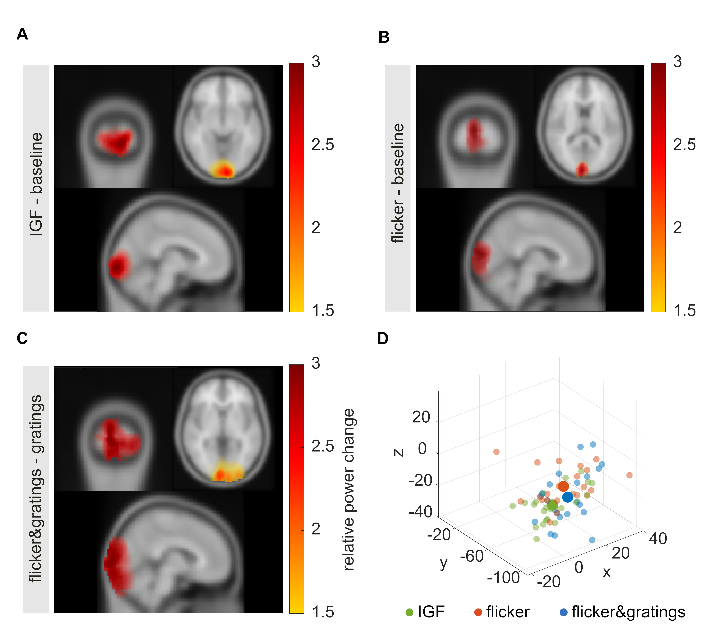
\includegraphics[width=116mm]{figures/fig10_sources_sq.eps}  
    \captionsetup{width=116mm}
    \caption[Source localization of the gamma oscillations and flicker response]{\textcolor{red}{Source estimates using the LCMV beamformer approach mapped on a standardized MNI brain. \textbf{A} Source estimation of the visually induced gamma oscillations (power change relative to baseline), with the peak of the source identified at MNI coordinates [-6mm -100mm -8mm]. \textbf{B} Source estimation of the flicker response (relative to baseline), with the average peak source at [6mm -96mm 12mm] (in Calcarine Fissure). \textbf{C} Source estimation of the flicker response in the \gammaRFT condition (relative to the gratings interval),  with the average peak source at [6mm -100mm 0mm] (in Calcarine Fissure). \textbf{D} Coordinates of the identified peak sources for all participants (small scatters) and grandaverage (large scatters) for the IGF, and the flicker responses in the \RFTonly and \gammaRFT condition (green, orange and blue, respectively). The peak sources of the flicker responses are adjacent to each other, while the gamma sources tend to peak at inferior locations.}}
    \label{fig:sourceGA}
\end{figure}}
\end{document}
